\documentclass{beamer}
\usetheme{JuanLesPins}
\usepackage[sort]{natbib}
\usepackage{graphicx}
\usepackage{subcaption}
\usepackage[linesnumbered,ruled,vlined]{algorithm2e}

% Add your references to the .bib file

% Components of the title page
\title[Comparison of Radix Sort and Tim Sort]{Comparison of Radix Sort and Tim Sort}
\subtitle{An Abstract}
\author[Tonmoy]{Tonmoy}
\institute[CSE, RUET]{CSE, RUET}
\date{\today}

\begin{document}

% Frame 1
\frame[plain]{\titlepage}

% Frame 2
\section*{Outline}
\frame[t]{
    \frametitle{Presentation Outline}
    \tableofcontents
}

% Frame 3
\section{Abstract}
\begin{frame}[t]
    \frametitle{Abstract}
    \cite{verma2013new}This paper presents a comparative analysis of Radix Sort and Tim Sort, two popular sorting algorithms. Radix Sort, a linear time, non-comparative algorithm, is explored with an enhanced version incorporating Counting Sort. Tim Sort, a hybrid algorithm combining Merge Sort and Insertion Sort, is detailed with a focus on its adaptability. The study aims to provide insights into their strengths, weaknesses, and optimal use cases.
\end{frame}

% Frame 4
\section{Introduction to Sorting Algorithms}
\subsection[Radix Sort]{Radix Sort Overview}
\begin{frame}[t]
    \frametitle{Introduction to Sorting Algorithms}
    \framesubtitle{Radix Sort Overview}
    Radix Sort is a linear time, non-comparative sorting algorithm that operates on integers by processing individual digits. It exhibits excellent performance for fixed-size integer keys and is known for its simplicity and efficiency in certain scenarios.\cite{shukla2012review}

    The time complexity of Radix Sort is linear, \(O(kn)\), where \(k\) is the number of digits in the input integers.
\end{frame}

% Frame 5
\subsection[Tim Sort]{Tim Sort Overview}
\begin{frame}[t]
    \frametitle{Introduction to Sorting Algorithms}
    \framesubtitle{Tim Sort Overview}
    Tim Sort, a hybrid sorting algorithm derived from Merge Sort and Insertion Sort, is designed for real-world data. Its ability to adapt to various scenarios, along with its efficiency in handling partially ordered data, makes it a popular choice in practice.

    The average-case time complexity of Tim Sort is \(O(n \log n)\), where \(n\) is the size of the input array.\cite{hammad2015comparative}
\end{frame}

% Frame 6
\section{Background Study}
\subsection{Radix Sort with Counting Sort}
\begin{frame}[t]
    \frametitle{Background Study}
    \framesubtitle{Radix Sort Pseudocode with Counting Sort\cite{hammad2015comparative}}
    \begin{algorithm}[H]
        \SetAlgoLined
        \KwData{Array $A$, Number of digits $d$}
        \For{$i \gets 1$ to $d$}{
            Use Counting Sort to sort array $A$ on digit $i$\;
        }
        \caption{Radix Sort with Counting Sort}
    \end{algorithm}
\end{frame}


% Frame 7
\subsection{Counting Sort}
\begin{frame}[t]
    \frametitle{Background Study}
    \framesubtitle{Counting Sort Pseudocode}
    \small
    \begin{algorithm}[H]
        \SetAlgoLined
        \KwData{Array $A$, Range of elements $k$}
        \KwResult{Sorted array $A$}
        $C \gets$ array of size $k$ initialized with zeros\;
        \For{$i \gets 1$ to $n$}{
            $C[A[i]] \gets C[A[i]] + 1$\;
        }
        \For{$i \gets 1$ to $k$}{
            $C[i] \gets C[i] + C[i-1]$\;
        }
        \For{$i \gets n$ to $1$}{
            $B[C[A[i]]] \gets A[i]$\;
            $C[A[i]] \gets C[A[i]] - 1$\;
        }
        \caption{Counting Sort}
    \end{algorithm}
\end{frame}

% Frame 8
\subsection{Tim Sort with Insertion Sort and Merge Sort}
\begin{frame}[t]
    \frametitle{Background Study}
    \framesubtitle{Tim Sort Pseudocode with Insertion Sort and Merge Sort\cite{jain2015bitonic}}
    \begin{algorithm}[H]
        \SetAlgoLined
        \KwData{Array $A$}
        \KwResult{Sorted array $A$}
        Divide the array into small blocks using Insertion Sort\;
        \While{blocks to merge}{
            Merge adjacent blocks using Merge Sort\;
        }
        \caption{Tim Sort with Insertion Sort and Merge Sort}
    \end{algorithm}
\end{frame}


% Frame 9
\subsection{Insertion Sort}
\begin{frame}[t]
    \frametitle{Background Study}
    \framesubtitle{Insertion Sort Pseudocode}
    \begin{algorithm}[H]
        \SetAlgoLined
        \KwData{Array $A$}
        \KwResult{Sorted array $A$}
        \For{$i \gets 2$ to $n$}{
            $key \gets A[i]$\;
            $j \gets i-1$\;
            \While{$j > 0$ and $A[j] > key$}{
                Swap $A[j+1]$ and $A[j]$\;
                $j \gets j-1$\;
            }
            $A[j+1] \gets key$\;
        }
        \caption{Insertion Sort}
    \end{algorithm}
\end{frame}

% Frame 10
\subsection{Merge Sort}

\begin{frame}[t]
    \frametitle{Background Study}
    \framesubtitle{Merge Sort Pseudocode (Part 1)}

    \begin{algorithm}[H]
        \SetAlgoLined

        \KwData{Array $A$, Indices $p$, $q$, $r$}
        \KwResult{Sorted array $A$}
        $n_1 \gets q - p + 1, n_2 \gets r - q$\;
        Create arrays $L[1..n_1+1]$ and $R[1..n_2+1]$\;
        \For{$i \gets 1$ to $n_1$}{
            $L[i] \gets A[p + i - 1]$\;
        }
        \For{$j \gets 1$ to $n_2$}{
            $R[j] \gets A[q + j]$\;
        }
        $L[n_1+1] \gets \infty, j \gets 1$\;
        $R[n_2+1] \gets \infty,i \gets 1$\;
        \caption{Merge Sort}
    \end{algorithm}
\end{frame}

\begin{frame}[t]
    \frametitle{Background Study}
    \framesubtitle{Merge Sort Pseudocode (Part 2)}

    \begin{algorithm}[H]
        \caption*{Merge Sort (continued)}
        \KwData{Array $A$, Indices $p$, $q$, $r$}
        \KwResult{Sorted array $A$ (continued)}
        \For{$k \gets p$ to $r$}{
            \If{$L[i] \leq R[j]$}{
                $A[k] \gets L[i]$\;
                $i \gets i + 1$\;
            }\Else{
                $A[k] \gets R[j]$\;
                $j \gets j + 1$\;
            }
        }
    \end{algorithm}
\end{frame}

% Frame 11
\section{Implementation of Radix Sort}
\begin{frame}[t]
    \frametitle{Implementation of Radix Sort\cite{anderson1998implementing}}

    \begin{itemize}
        \item \textbf{Input:} Array $A$
        \item \textbf{Output:} Sorted array $A$ using Radix Sort
        \item Find the maximum number of digits, $d$, in elements of $A$
        \item \textbf{For} $i$ from $1$ to $d$:
              \begin{itemize}
                  \item Use Counting Sort to sort array $A$ based on the $i$-th digit
              \end{itemize}
    \end{itemize}

    \begin{figure}
        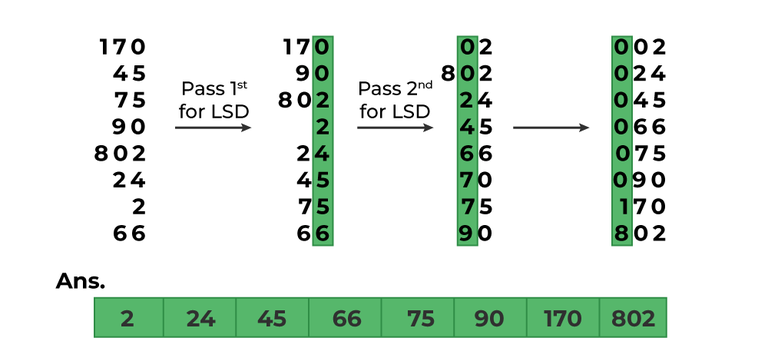
\includegraphics[width=0.7\linewidth]{radix_sort.png}
        \caption{Radix Sort Visualization}
    \end{figure}
\end{frame}

% Frame 12
\section{Implementation of Tim Sort}
\begin{frame}[t]
    \frametitle{Implementation of Tim Sort}

    \begin{itemize}
        \item \textbf{Input:} Array $A$
        \item \textbf{Output:} Sorted array $A$ using Tim Sort
        \item Divide the array into small blocks using Insertion Sort
        \item \textbf{While} there are blocks to merge:
              \begin{itemize}
                  \item Merge adjacent blocks using Merge Sort
              \end{itemize}
    \end{itemize}

    \begin{figure}
        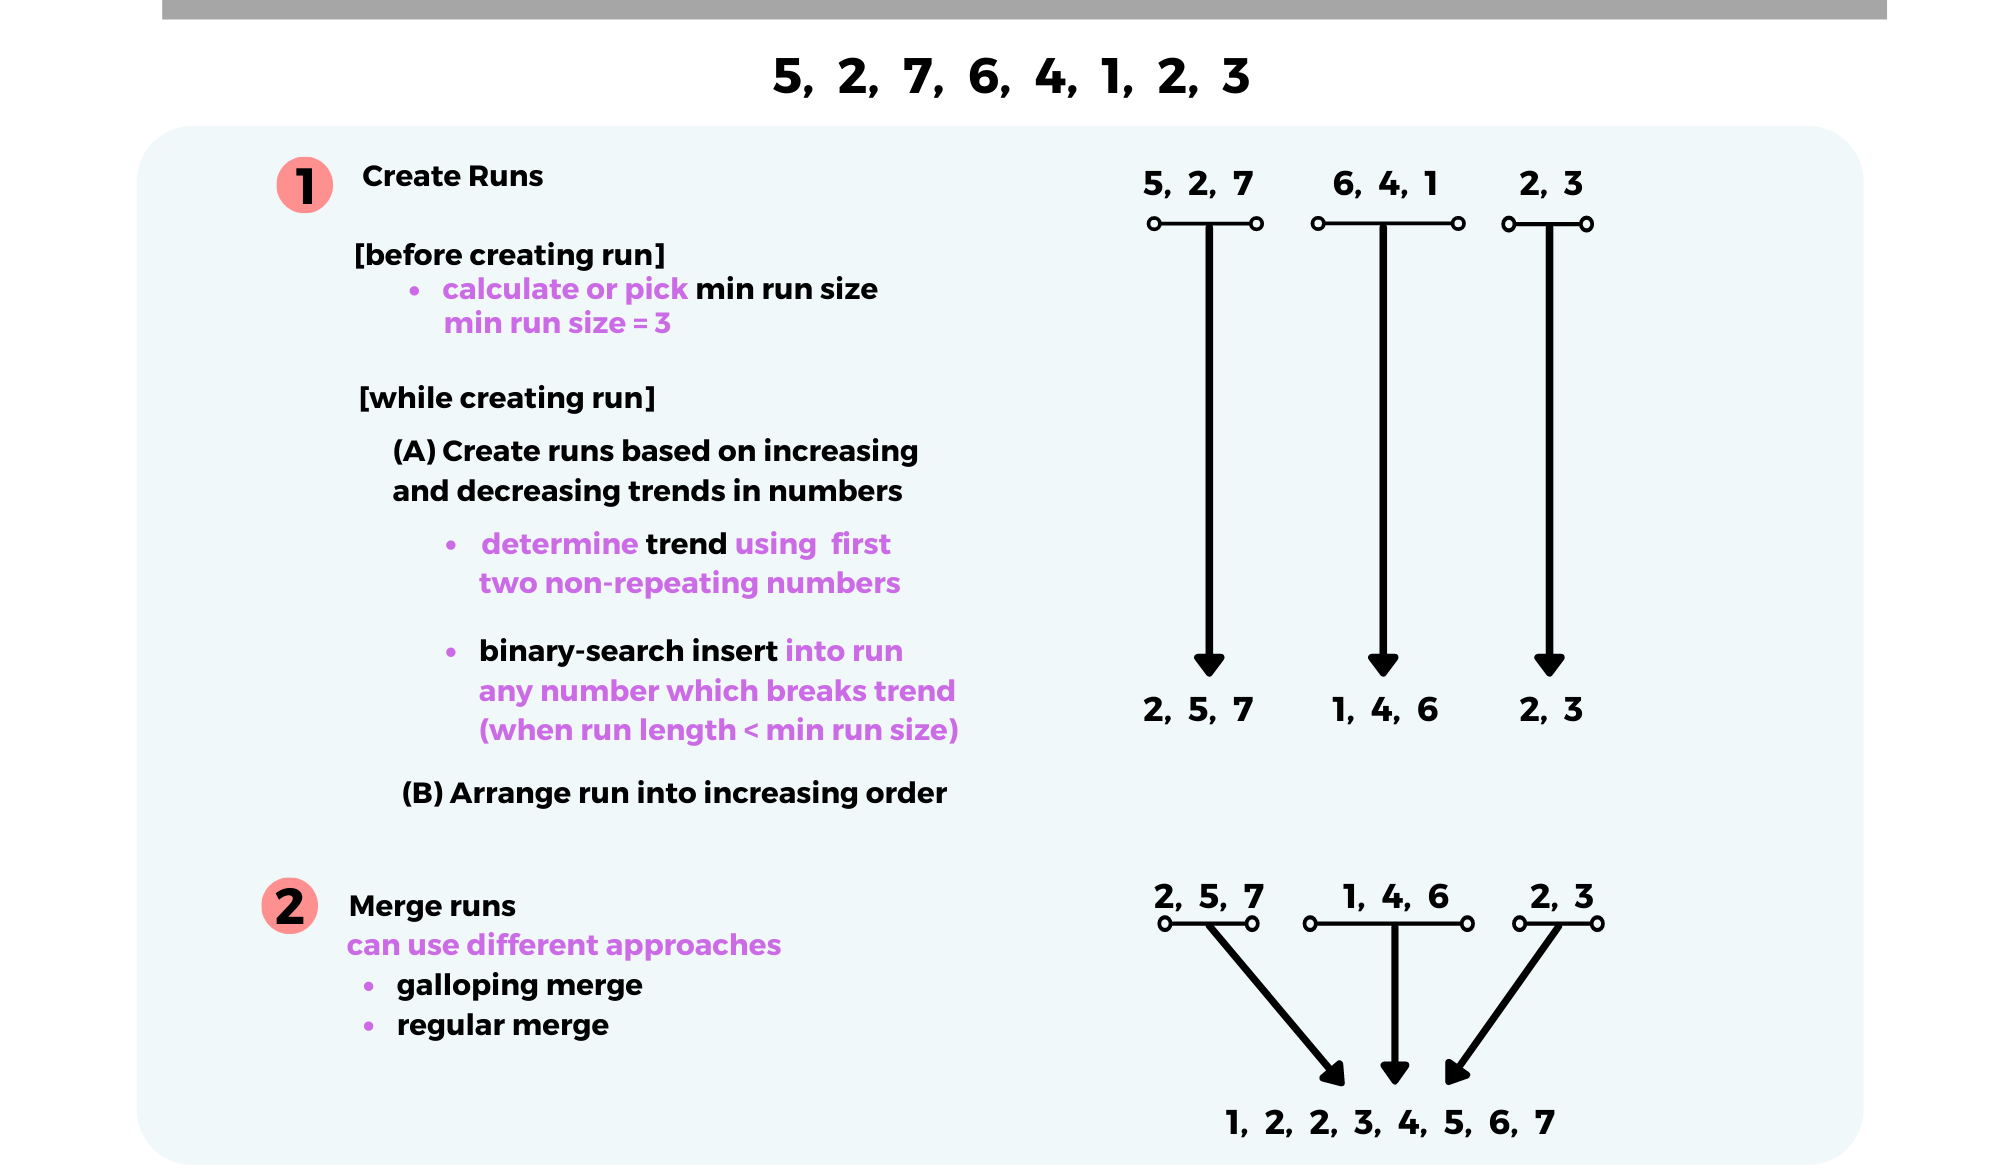
\includegraphics[width=0.5\linewidth]{tim_sort.png}
        \caption{Tim Sort Visualization}
    \end{figure}
\end{frame}

%Frame 13
\section{Results and Analysis}

\begin{frame}{Comparison Table}

    \begin{table}[h]
        \caption{Comparison between Timsort and Radix Sort}
        \begin{tabular}{|p{2.3cm}|p{4cm}|p{4cm}|}
            \hline
            \textbf{Topics}                                                                                         & \textbf{Radix Sort} & \textbf{Timsort} \\
            \hline
            \textbf{Time Complexity}                                                                                & $O(nk)$             & $O(n \log n)$    \\
            \hline
            \textbf{Space Complexity}                                                                               & $O(n + k)$          & $O(n)$           \\
            \hline
            \textbf{Application }                                                                                   &
            \begin{minipage}[t]{\linewidth}
                Sorting items of fixed-length.\\
                Sorting strings where product of the length of the largest item is and number of item is not too large.
            \end{minipage} &
            \begin{minipage}[t]{\linewidth}
                \cite{sahni2011gpu}Timsort is a hybrid sorting algorithm derived from merge sort and insertion sort.\\
                Where is a balance between time and space complexity is desired.
            \end{minipage}                                              \\
            \hline
        \end{tabular}
    \end{table}
\end{frame}



% Frame 14
\section{Results and Analysis}

\begin{frame}{Time complexity}
    \begin{figure}[h]
        \centering
        \begin{subfigure}{.49\textwidth}
            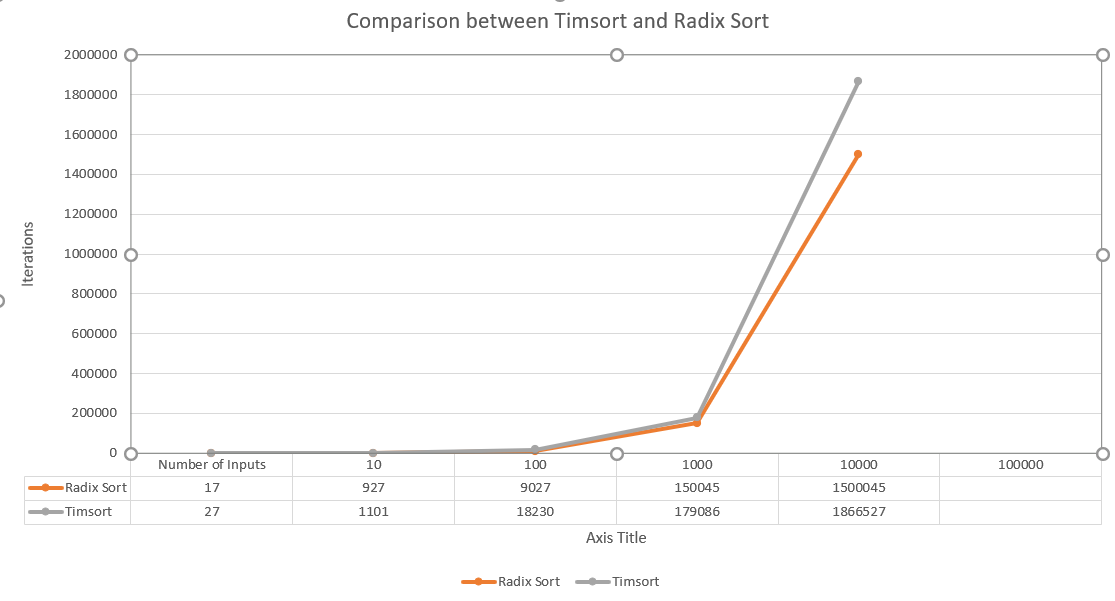
\includegraphics[width=\linewidth]{chart.png}
            \caption{Chart Comparison}
            \label{fig:subfig1}
        \end{subfigure}
        \hfill
        \begin{subfigure}{.49\textwidth}
            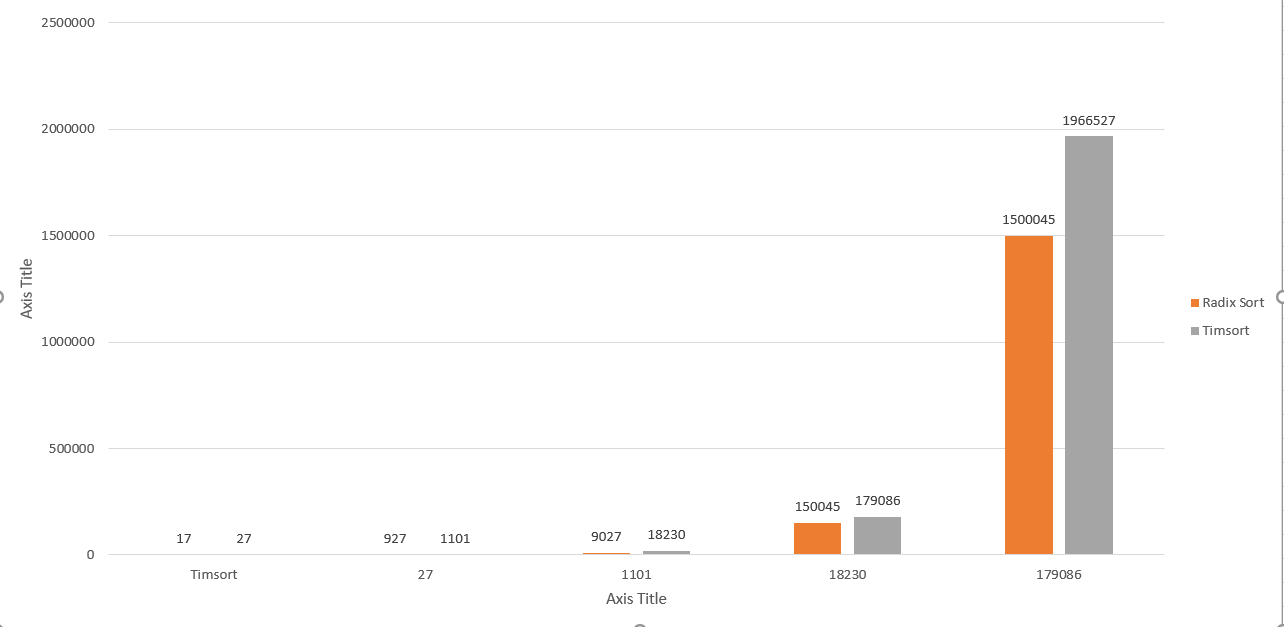
\includegraphics[width=\linewidth]{bar.png}
            \caption{Bar Comparison}
            \label{fig:subfig2}
        \end{subfigure}
        \caption{Comparison between Timsort and Radix Sort.}
        \label{fig:both}
    \end{figure}
\end{frame}

% Frame 15

\begin{frame}{Time complexity}
    \begin{table}[h]
        \centering
        \caption{Comparison between Radix Sort's and Timsort's iterations}
        \begin{tabular}{|c|c|c|}
            \textbf{Number of Inputs} & \textbf{Radix Sort} & \textbf{Timsort} \\
            \hline
            10                        & 17                  & 27               \\
            \hline
            100                       & 927                 & 1101             \\
            \hline
            1000                      & 9027                & 18230            \\
            \hline
            10000                     & 150045              & 179086           \\
            \hline
            100000                    & 1500045             & 1666527          \\
            \hline
        \end{tabular}
    \end{table}
    \begin{enumerate}
        \item Radix Sort's time complexity is almost similar to $O(n * k)$, where $n$ stands for the number of items in the data set, and $k$ is the length of the longest number in the data set.
        \item Timsort's time complexity is almost similar to $O(n log n)$, where $n$ stands for the number of items in the data set\cite{khairullah2013enhancing}.

    \end{enumerate}
\end{frame}

% Frame 16
% Conclusion Section
\section{Conclusion}

\begin{frame}{Conclusion}
    \begin{itemize}
        \item In conclusion, Radix Sort and Timsort are both effective sorting algorithms, each with its own strengths and use cases.

              \textbf{Radix Sort:}
              \begin{itemize}
                  \item Radix Sort demonstrates efficiency in scenarios where the range of input values is not significantly larger than the number of elements.
                  \item With a time complexity of $O(n \cdot k)$, where $n$ is the number of elements and $k$ is the length of the longest digit.\cite{alkharabsheh2013review}
              \end{itemize}

              \textbf{Timsort:}
              \begin{itemize}
                  \item Timsort, a hybrid sorting algorithm derived from merge sort and insertion sort, exhibits a time complexity of $O(n \log n)$.
              \end{itemize}
    \end{itemize}
\end{frame}
% Frame 17
\section{References}

\begin{frame}[allowframebreaks]{References}
    \bibliographystyle{plain}
    \bibliography{ref}
\end{frame}

\end{document}
